\documentclass{beamer}
\usepackage[bookmarks=true]{hyperref}
\usepackage{subfig}

\mode<presentation> {
	\usetheme{Madrid}
	\usecolortheme{rose}
}


\title[An Image is Worth 16x16 Words]{An Image is Worth 16x16 Words: \\ Transformers for Image Recognition at Scale}
\author{Koorye}
\institute[UESTC]{University of Electronic and Science Technology of China}
\date{13th May 2024}

\begin{document}

\begin{frame}
\titlepage
\end{frame}

\begin{frame}
\frametitle{Outline}
\tableofcontents
\end{frame}

\section{Research Aim}

\begin{frame}
\frametitle{Research Aim}

\textbf{The GAP between Language Models and Vision Models:}

\begin{figure}
\centering
\subfloat[Language Model receives 1D sequence]{
	\begin{minipage}[b]{160pt}
		\centering
		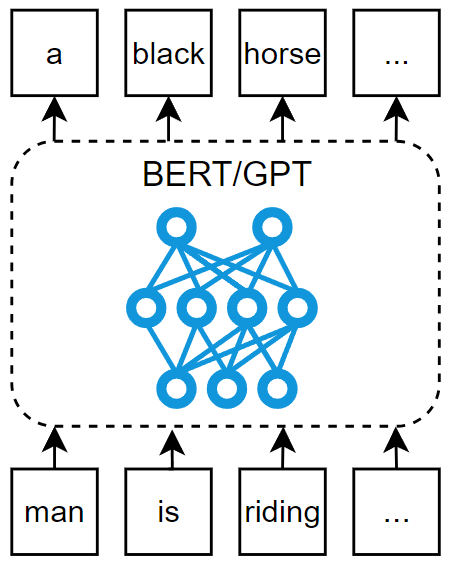
\includegraphics[width=100pt]{pics/bert_gpt.png}
	\end{minipage}
}
\subfloat[Vision Model receives 2D image pixels]{
	\begin{minipage}[b]{160pt}
		\centering
		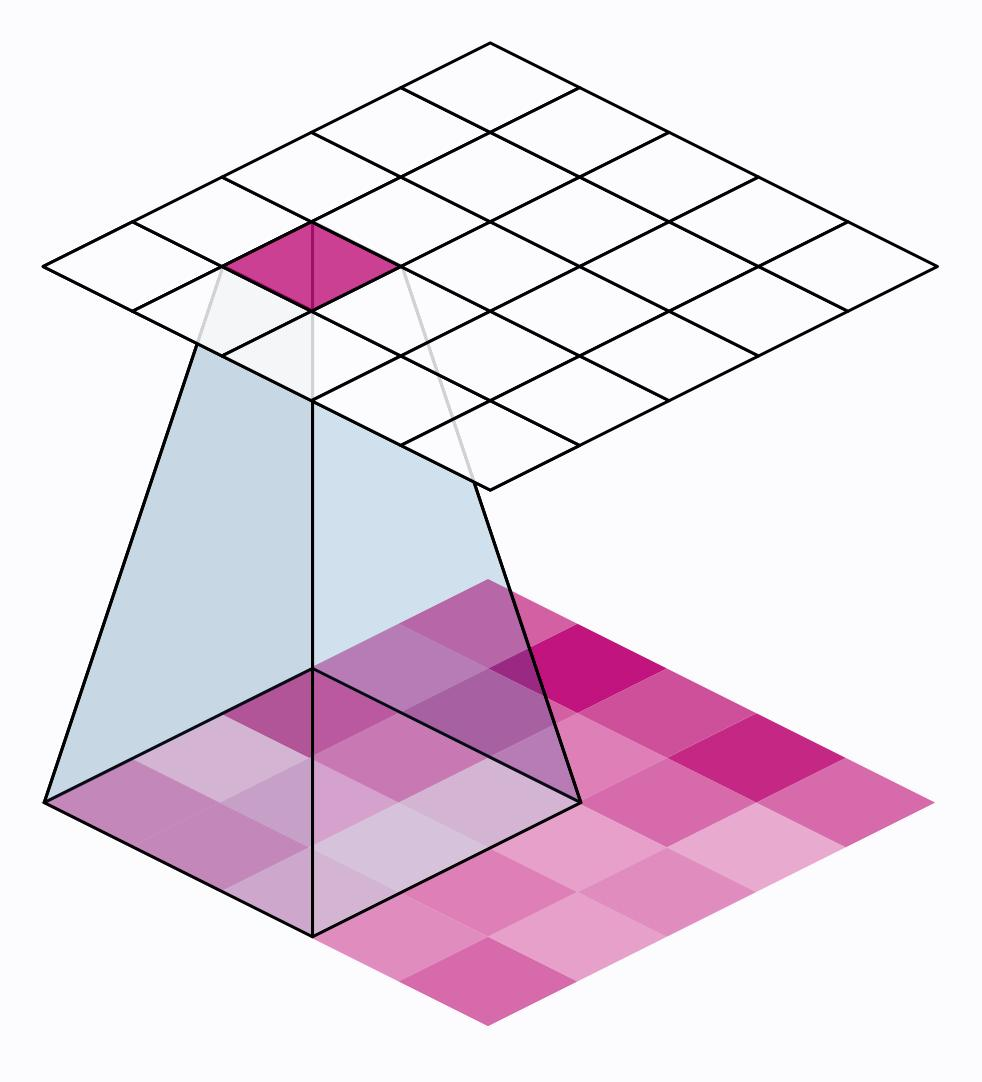
\includegraphics[width=100pt]{pics/conv.jpg}
	\end{minipage}
}
\end{figure}

\textbf{Could the approach used in Language Models inspire a new era for visual tasks?}

\end{frame}

\section{Method}

\begin{frame}
\frametitle{Method}

\begin{figure}
\centering
\subfloat[Vision Transformer Model]{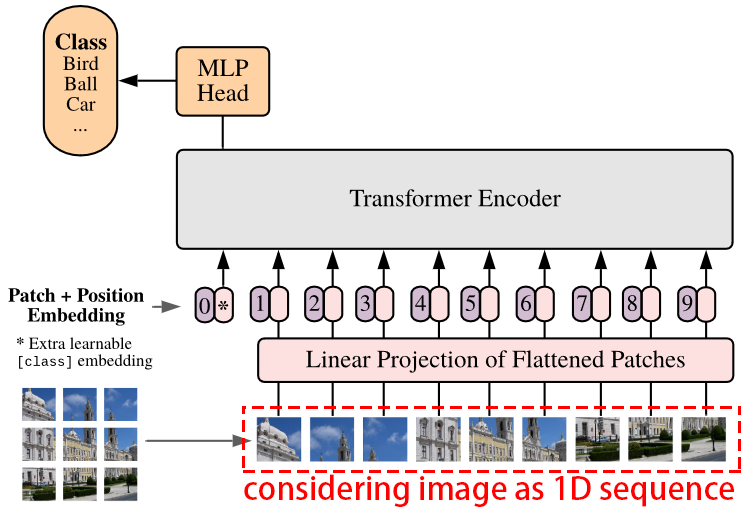
\includegraphics[width=150pt]{pics/vit.png}}
\hspace*{50pt}
\subfloat[Attention Module]{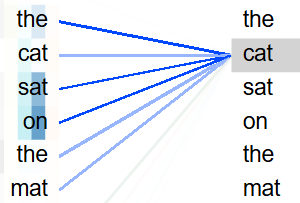
\includegraphics[width=100pt]{pics/attention.png}}
\end{figure}

\begin{itemize}
	\item Considering images as \textbf{1D sequences} of patches, like text sentences.
	\item Model the \textbf{relationship} between patches, like the process of human understanding.
\end{itemize}

\end{frame}

\section{Results}
\begin{frame}
\frametitle{Results}

\begin{figure}
\centering
\subfloat[Model Accuracy Comparison]{
	\begin{minipage}[b]{160pt}
		\centering
		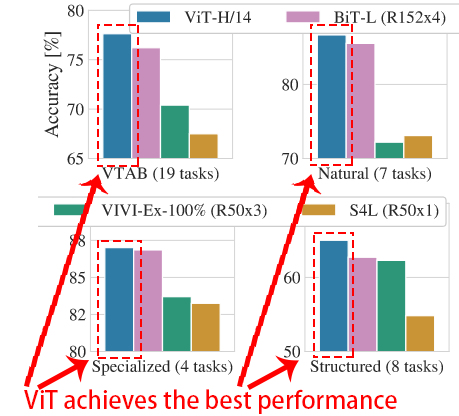
\includegraphics[width=130pt]{pics/acc.png}
	\end{minipage}
}
\subfloat[Attention Viusalization]{
	\begin{minipage}[b]{160pt}
		\centering
		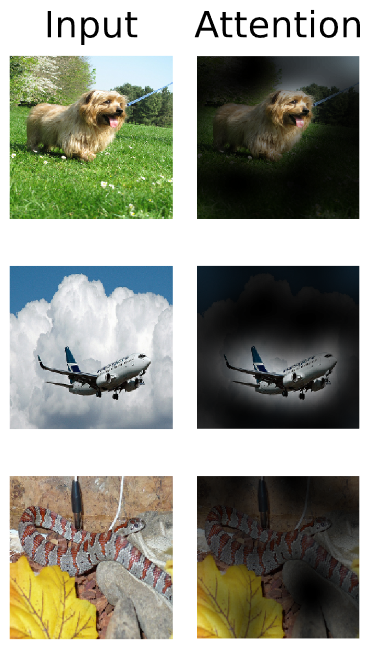
\includegraphics[width=70pt]{pics/attention_viz.png}
	\end{minipage}
}
\end{figure}

\begin{itemize}
	\item The \textbf{accuracy} of model reaches a new level with smaller model \textbf{size}.
	\item Attention modules capture \textbf{visually rich areas} of information.
\end{itemize}

\end{frame}

\section{Conclusion \& Discussion}
\begin{frame}
\frametitle{Conclusion \& Discussion}

\textbf{Conclusion:}

\begin{itemize}
	\item Inspired by Language Models, processing images into sequences similar to text.
	\item Surpassing traditional models in accuracy and being more compact.
\end{itemize}

\bigskip
\bigskip

\textbf{Discussion:}

\begin{itemize}
	\item Need more training data and larger models to maximize its potential.
	\item Unknown performances in more visual tasks.
\end{itemize}

\end{frame}

\end{document}